\chapter{Brief Introduction}
\section{HTML Fetch}

Bear with the start as we go run through a bit of history with browser requests and page loads, and know we will quickly move into REST examples and get into our case study.

Diving right in, I have a TCP packet capture intercepting traffic on port 8080.  I'm running an nginx docker container, which is serving a single index.html static page at \url{http://localhost:8080/index.html}. Ignore docker, ignore port 8080, ignore nginx, just know that on my local machine I have a service running which works like any website and am capturing the request and response between my browser and the local service.

\begin{sidebar}
\begin{minipage}{\linewidth}
\begin{center}
\textbf{Demo Execution}
\end{center}
Performing this demo locally isn't required, but if you're curious, you can.  First step is to create a simple index.html page with any text editor that contains "hello world".  You can serve this index.html page up using an nginx container with
\begin{code}
\begin{lstlisting}[belowskip=-\baselineskip]
docker run --name local-nginx -p 8080:80 \
-v /tmp/static:/usr/share/nginx/html:ro -d nginx
\end{lstlisting}
\end{code}
Which assumes the index.html is on your local machine at \textit{/tmp/static/index.html}. Finally, the packet capture can be performed from a BASH command line such as WSL or MacOS Terminal.
\begin{code}
\begin{lstlisting}[belowskip=-\baselineskip]
sudo tcpdump -i eth0 -s0 -w demo.pcap port 8080
\end{lstlisting}
\end{code}
With these quick steps, we have an HTML page available from an nginx container running on 8080, with packet captures being appended to demo.pcap.
\end{minipage}
\end{sidebar}

Opening my FireFox browser to \url{http://localhost:8080/index.html}, I receive my "hello world" reply.  Halting the packet capture with \textit{CTRL+C}, I now have a packet capture I can open with WireShark.

\begin{sidebar}
\begin{center}
\textbf{Don't Use WireShark at Work}
\end{center}
I discovered the hard way that WireShark may get you in trouble from overzealous IT admins in the workplace.  WireShark defaults to running in promiscuous mode, which allows you to capture any traffic your network interface card (NIC) receives, which may include unencrypted traffic intended for other receivers.  Some work environments monitor for services running in promiscuous mode, attempting to identify network adversaries (hackers) and corporate espionage.  Other workplaces monitor for installations of WireShark and other hacker-friendly tools.  I recommend avoiding WireShark installations without explicit written approval.
\end{sidebar}

Examining the packet capture, we can see the following traffic:

\textit{Browser client to server:}

\begin{code}
\vspace{-\baselineskip}
\begin{lstlisting}[belowskip=-\baselineskip]
GET / HTTP/1.1
Host: localhost:8080
User-Agent: Mozilla/5.0 (Windows NT 10.0; Win64; x64; rv:83.0) Gecko/20100101 Firefox/83.0
Accept: text/html,application/xhtml+xml,application/xml;q=0.9,image/webp,*/*;q=0.8
Accept-Language: en-US,en;q=0.5
Accept-Encoding: gzip, deflate
DNT: 1
Connection: keep-alive
Upgrade-Insecure-Requests: 1
\end{lstlisting}
\end{code}

\textit{Server response:}

\begin{code}
\vspace{-\baselineskip}
\begin{lstlisting}[belowskip=-\baselineskip]
HTTP/1.1 200 OK
Server: nginx/1.19.5
Date: Mon, 14 Dec 2020 03:31:55 GMT
Content-Type: text/html
Content-Length: 12
Last-Modified: Mon, 14 Dec 2020 00:06:19 GMT
Connection: keep-alive
ETag: "5fd6ac7b-c"
Accept-Ranges: bytes

hello world
\end{lstlisting}
\end{code}

From the client initial request, we have \textit{GET / HTTP/1.1} which indicates the HTTP Method of \textit{GET}, the resource requested \textit{/}, and the protocol and protocol version \textit{HTTP 1.1}.  Following the method, resource, and protocol, we have a list of key-value pairs known as HTTP headers indicating our language, our client, what the target host is, and more.

From the server reply, we have a similar \textit{HTTP/1.1 200 OK} which tells us the protocol version we're replying with, a status code of \textit{200 OK}, followed by similar key-value pairs of headers which tells us information about the server, how big the server reply is, when it was last modified, and the type of content being returned.  Finally, we have the body of the request which includes the text placed into index.html of \textit{hello world}.

To understand REST and how it works, it is important to grasp that we are moving towards conventions of these resources, status codes, bodies, methods, and headers to map out a plan for transferring state of resources.  In the crash course introduction for REST:
\begin{itemize}
  \item The Uniform Resource Locator (URL) identifies the target object or collection of objects.  For example a URL of \textit{/v1/books/123-567} may be a fetch of a book with ISBN 123-567.
  \item The HTTP status code tells you if the operation succeeded or failed.  For example, \textit{201 Created} tells you a resource was Created.
  \item The HTTP headers convey context both for the client and for the server.  Context is anything outside of the object state being retrieved or modified, such as user or browser.
  \item The body conveys the current state, the state to change to, or the edit being requested.
\end{itemize}

\section{What is REST?}

For the textbook answer, REST is short for Representational State Transfer, an architectural pattern for HTTP web services that was originally presented by Roy Fielding in 2000 \cite{fielding}.  Over time it has transitioned into transactional-like definition of services, playing to the dynamic needs of web content and native clients.  For those who grimace at the "transactional-like", your status codes are your error code / success code equivalent, and still I'm sure some readers will gag at the notion.

At its heart, REST describes convention of CRUD (create, read, update, delete) operations into standardized methods.  REST is another step forward in the convention-over-configuration direction that developers started when moving from build scripts written in ANT XML to Maven and Gradle.  Status codes dictated by W3C committees are used to quickly convey success/failure.  Headers are used to carry context instead of state, including identity and authorization.  Target state is transferred to the server via the request body, and the result state is transferred to the client in the result body.

If you've ever tried to use native protocols, or someone's home-grown socket solution, you'll appreciate the consistent feel of a well-written REST API.

\section{We tried this before...}

A bit of history to understand some of the legacy any engineer facing enterprise problems will likely encounter.  For those thinking everyone has moved to microservices, your banks still manage your money in mainframes, and most of your flights are managed through SOAP.  COBOL is still in use today, and don't be fooled thinking history won't find a way to make your life miserable at some point in your career.  Legacy code manages to employ a lot of our peers.  If you're a Java developer, you're going to encounter old-school Java Servlet Pages (JSPs), Web-ARchives (WARs), and Enterprise Application aRchives (EARs).  You're welcome.

WEB 1990s and early 2000s architecture was structured like this:

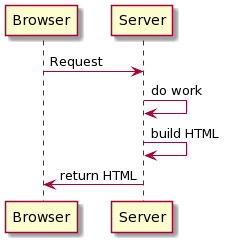
\includegraphics{browserToServer}

The browser would request a web page and the server would do some work to hand build it.  Inevitably as more browsers came online, and more browser versions came online, more and more work had to be performed by the server developers to tailor to issues with content rendering in various browsers. Mostly fighting Internet Explorer.  Additionally, as web content became more and more complex, so did the code to build the customized reply for shopping carts, bank statements, flight status, etc.

Eventually, server developers started adopting frameworks such as ASP.NET (C++) or JSPs (Java) which isolated built parameters with HTML response content:

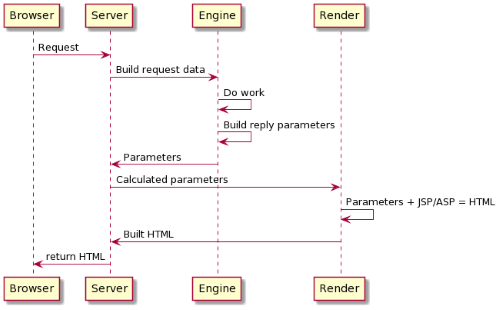
\includegraphics{jsps}

Anyone with experience building JSPs and ASPs knows it actually works a little different, such as JSP and Java getting compiled into a single .class file which is treated as both the renderer and the engine, but for the history lesson, the process is more important than the actual artifact.

With this update, we began the process of isolating calculated output from the rendered view.  It was our first step into MVC (Model-View-Controller), but we still faced issues of page content becoming more and more complex being tailored to more and more browsers.  More than that, we had a nasty problem of scale.  In this situation, the server receiving the request would have to do the work, build the page, and fire the reply in a timely manner.  To scale, we needed to enable server-to-server communication.

Our first dive into server-to-server involved custom socket buffer definitions, which then migrated into Simple Object Access Protocol, aka SOAP.

\begin{sidebar}
\begin{center}
\textbf{XML, SOAP, and JSON}
\end{center}
We're going to hit on a bit of history with XML, SOAP, and JSON so it is worth having a short example of each as a TODO list.

Sample XML reply that could be considered "browser friendly":

\begin{code}
\vspace{-\baselineskip}
\begin{lstlisting}[belowskip=-\baselineskip]
<?xml version="1.0" encoding="UTF-8"?>
<todo>
  <item>Laundry</item>
  <item>Trash</item>
  <item>Dishes</item>
</todo>

\end{lstlisting}
\end{code}

With a potential SOAP equivalent:

\begin{code}
\vspace{-\baselineskip}
\begin{lstlisting}[belowskip=-\baselineskip]
<?xml version = "1.0" encoding="UTF-8"?>
<SOAP-ENV:Envelope
   xmlns:SOAP-ENV = "http://www.w3.org/2001/12/soap-envelope"
   SOAP-ENV:encodingStyle = "http://www.w3.org/2001/12/soap-encoding">

   <SOAP-ENV:Body xmlns:m = "https://www.example.com/todos">
      <m:Todo>
         <m:Item>Laundry</m:Item>
         <m:Item>Trash</m:Item>
         <m:Item>Dishes</m:Item>
      </m:Todo>
   </SOAP-ENV:Body>
</SOAP-ENV:Envelope>

\end{lstlisting}
\end{code}

Finally, our less-verbose, browser and user-friendly JSON equivalent:

\begin{code}
\vspace{-\baselineskip}
\begin{lstlisting}[belowskip=-\baselineskip]
{"todo": ["Laundry", "Trash", "Dishes"]}
\end{lstlisting}
\end{code}

\end{sidebar}

SOAP has a rather lengthy and sordid history, which is not the focus of this book, but it is worth touching upon.  SOAP was a rather loose concept of standardizing XML, conveying context such as username and passwords, the request, and the action being performed.  All of it was XML and different architects would inevitably have very different approaches.  Context information such as session, user, password, and more could be found as HTTP Headers, within the SOAP Envelope, or even within the SOAP Body.  SOAP was verbose, machine-friendly, JavaScript unfriendly, not very developer-friendly, and fragmented.  There are certainly more issues with SOAP, but you get the point.

\begin{minipage}{\linewidth}
So, with SOAP, we migrated an XML API architecture approaching something along the lines of

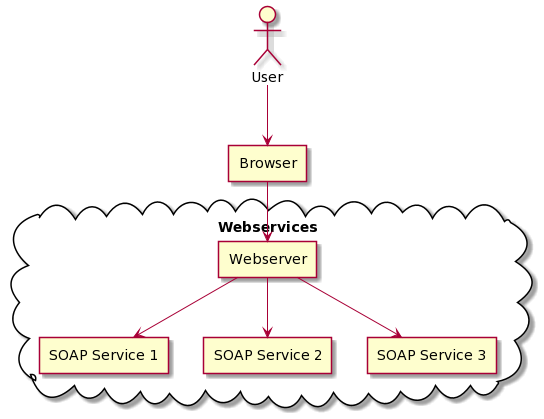
\includegraphics{soap1}

\end{minipage}

This is still before mobile phones are a thing.  The web continues to grow and users are loading up Netscape, Internet Explorer, Opera, FireFox, and others.  Content started to not only require different HTML responses but different release cycles outside of the SOAP service development cycle.  Offering up media such as CSS and image changes took an isolated release process from many of the SOAP services.  Enter Asynchronous JavaScript and XML, better known as AJAX.  AJAX + SOAP really was too much to handle, as you started to see ugly JavaScript needing to be written to handle the SOAP payloads.  More often, you'd have custom XML services talking to custom SOAP and databases.

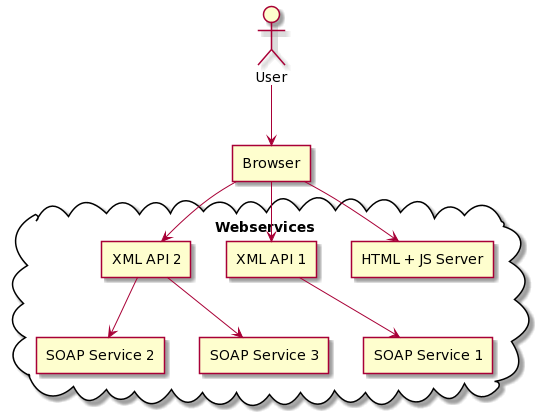
\includegraphics{soap2}

The problem compounds as the page complexity grows and now you have browser-friendly XML APIs and server SOAP APIs.  Inevitably the clients on both browsers and servers, for browser-to server and server-to-server communication needs to become more consistent and more consumer friendly.  Concurrently to all of this nasty fragmentation, browser engineers start forcing the issue with JavaScript Object Notation (JSON).

In quick succession, smart (and staffed) companies pull this stunt:

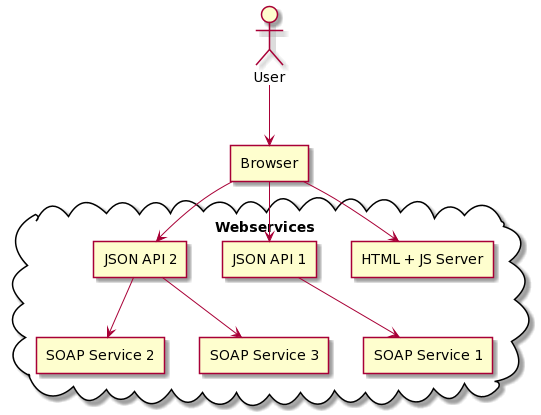
\includegraphics{js1}

followed by

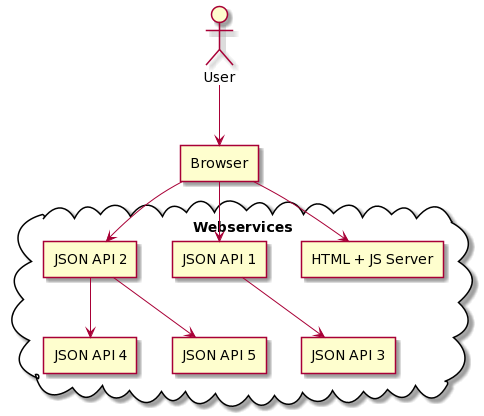
\includegraphics{js2}

Next step was just to standardize the JSON APIs, getting to that convention-over-configuration that offers enough consistency to feel common but malleable enough to answer business requirements without feeling like hammering a square peg into a round hole.  REST is the chosen victor in our arena.

Ultimately, it rapidly progresses into something luxurious that supports mobile clients, browser clients, internal server-clients, customer servers, API gateway proxies, geo-distributed content delivery networks (CDNs), with RESTful APIs providing the majority of server-state to all interested consumers.

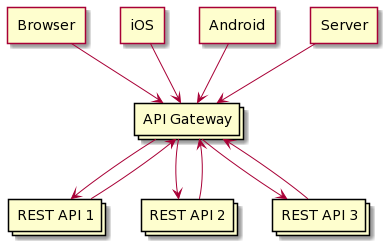
\includegraphics{modern}

\begin{sidebar}
\begin{center}
\textbf{Hidden Services}
\end{center}

Do note, this diagram is completely missing big ticket items like scalable block storage, databases, eventing systems, messaging systems, and more.  The point being made is that client-to-server and server-to-server communication channels moved from fragmented APIs and standards to consistent channels of REST communication.

\end{sidebar}

\section{Case Study: Library}

Throughout the remainder of this text, we will leverage a case study to design an API with the Open API 3.0 specification.  Our project is to design an API for administrators and consumers of a library.  User stories will include book check-in, book check-out, lost books, sold books, and book availability.  The list of user stories is offered here to allow you to have foresight into where we will take this project, but it is not required you go through them now.  Certainly, don't get ahead of yourself and begin planning out the API just yet.

\begin{itemize}
  \item I as a Borrower need to check on a book's availability so that I may know if the book I wish to checkout is available.
  \item I as a Borrower need to search for a book by title so that I may know if the book I wish to checkout is available.
  \item I as an Admin need to reserve a copy of a book for a patron so that they may know it is available when they arrive.
  \item I as an Admin need to create a book so that I may prepare incoming purchased books for borrowing.
  \item I as an Admin need to mark a book as sold so that I may remove sold book copies.
  \item I as an Admin need to create a borrower account so that I may enable new borrowers.
  \item I as an Automated System need to find past-due books so that I may notify borrowers of fines and fees.
\end{itemize}

Obviously, this list is entirely incomplete of what services would be required for a full library service offering.  You'd need user search features, account administration features, administrator administration features, payment services, and more.

Our identified actors include:

\begin{itemize}
  \item Admin: Your friendly librarian.
  \item Borrower: Anyone interested in checking out books.
  \item Automated System: A running application or batch process; just code that does regular work be it scheduled or on-demand.
\end{itemize}
